\section{Vehicle, Stages and Mission}
\label{sec:vehicle}

The simulator follows the Falcon 9 launch vehicle in the configuration flown
on SpaceX CRS-10, the tenth Commercial Resupply Services mission to the
International Space Station (launched 19 February 2017 from Launch
Complex~39A; the first stage returned to a landing site near the pad)
\cite{nasacrs10press}. The model is not a reconstruction of flight
hardware: it is a project-configured representation assembled from
published sources. Every adopted parameter value therefore carries an
evidence class --- K (authoritative known value), E (literature estimate)
or A (explicit modeling assumption) --- and the tables in this report state
the class of every value. The underlying records are
\texttt{data/vehicle\_parameters.json} (parameter set and sources) and
\texttt{data/crs10\_mission.json} (mission configuration).

\subsection{Vehicle configuration and stages}

The modeled vehicle is a two-stage stack of $62.4\,\mathrm{m}$ model height:
stage~1 ($42.6\,\mathrm{m}$), stage~2 ($12.6\,\mathrm{m}$), and the
Dragon~spacecraft with its trunk represented as one uniform assembly of
$7.2\,\mathrm{m}$ equivalent length and $1.83\,\mathrm{m}$ equivalent
radius. All axial stations are measured from the structural base of the
referenced stage along the vehicle's Body $+x$ axis (toward the nose).
Table~\ref{tab:vehicle} lists the adopted geometry and mass values.

\begin{table}[htbp]
\centering
\begin{tabular}{lrl}
\toprule
Component & Value & Class \\
\midrule
Outer diameter & $3.66\,\mathrm{m}$ & K \\
Stage-1 length & $42.6\,\mathrm{m}$ & E/A \\
Stage-2 length & $12.6\,\mathrm{m}$ & E/A \\
Dragon$+$trunk equivalent length & $7.2\,\mathrm{m}$ & E/A \\
Model total height & $62.4\,\mathrm{m}$ & E/A \\
Stage-1 dry mass & $22\,200\,\mathrm{kg}$ & E \\
Stage-1 propellant load & $410\,900\,\mathrm{kg}$ & E \\
Stage-2 dry mass & $4\,000\,\mathrm{kg}$ & E \\
Stage-2 propellant load & $107\,500\,\mathrm{kg}$ & E \\
Dragon loaded assembly (incl.\ cargo) & $8\,430\,\mathrm{kg}$ & E \\
Launch mass (model sum) & $553\,030\,\mathrm{kg}$ & E/A \\
Stage-1 dry CG station above base & $17.52\,\mathrm{m}$ & E/A \\
Stage-1 dry inertia $[I_{xx},I_{yy},I_{zz}]$ & $[61\,368.59, 4\,441\,994.04, 4\,441\,994.04]$\,$\mathrm{kg\,m^2}$ & E/A \\
\bottomrule
\end{tabular}
\caption{Vehicle geometry and mass model with evidence classes. Stage
lengths combine legacy Full Thrust geometry with a contiguous-stage model;
the Dragon assembly mass (including $2\,490\,\mathrm{kg}$ of cargo
\cite{nasacrs10overview}) is an external estimate
\cite{kyledatasheet}. Sources: geometry and dry/propellant masses
\cite{spacexguide2025,pezent2024,crs1presskit}.}
\label{tab:vehicle}
\end{table}

Inside stage~1, the RP-1 tank occupies the axial interval
$x = 4.0$--$18.7\,\mathrm{m}$ and the LOX tank $x = 18.7$--$40.8\,\mathrm{m}$;
the liquids are modeled as settled flat cylinders at constant densities
($820\,\mathrm{kg/m^3}$ for RP-1, $1\,250\,\mathrm{kg/m^3}$ for LOX). The
stage-1 dry mass contains a residual hardware budget of $6\,450\,\mathrm{kg}$
distributed uniformly over $x = 4.0$--$40.8\,\mathrm{m}$, since no surveyed
location exists; if that budget were free to move within its interval, the
dry CG station would shift between $12.18\,\mathrm{m}$ and $22.87\,\mathrm{m}$.
This range is a conditional spread of the placement assumption, not a
confidence interval. Tank geometry, depletion and the resulting CG and
inertia migration are treated in the propulsion and mass model chapter of
this report.

\subsection{Propulsion inventory}

Stage~1 carries nine Merlin 1D SL engines on a $1.3\,\mathrm{m}$ radius
ring (A); stage~2 carries a single MVac engine. Engine thrust application
(pivot) stations are $1.0\,\mathrm{m}$ and $0.5\,\mathrm{m}$ above the
respective stage base (A), and the gimbal limit is
$5^{\circ}$ (A). The model derives the vacuum thrust from the historical
sea-level operating point of $756\,\mathrm{kN}$ per engine
\cite{spacex2015} using the nozzle exit area $A_e$ and sea-level pressure
$p_0 = 101\,325\,\mathrm{Pa}$:
%
\begin{equation}
\label{eq:thrust-vac}
T_{\mathrm{vac}} = T_{\mathrm{sl}} + A_e \, p_0,
\qquad
I_{\mathrm{sp,sl}} = I_{\mathrm{sp,vac}} \, \frac{T_{\mathrm{sl}}}{T_{\mathrm{vac}}}
\end{equation}
%
which yields $824.901\,\mathrm{kN}$ and $285.023\,\mathrm{s}$
(respectively $935\,\mathrm{kN}$ and $348\,\mathrm{s}$ for the
literature-sourced MVac). Table~\ref{tab:engines} summarizes the engine set;
none of these values is a certified CRS-10 engine rating.

\begin{table}[htbp]
\centering
\begin{tabular}{lcc}
\toprule
Parameter & Merlin 1D SL ($\times 9$) & MVac ($\times 1$) \\
\midrule
Sea-level effective thrust & $756.000\,\mathrm{kN}$ (E/A) & --- \\
Vacuum thrust & $824.901\,\mathrm{kN}$ (E/A) & $935\,\mathrm{kN}$ (E) \\
Vacuum specific impulse & $311\,\mathrm{s}$ (E) & $348\,\mathrm{s}$ (E) \\
Sea-level specific impulse & $285.023\,\mathrm{s}$ (E/A) & --- \\
Nozzle exit area & $0.68\,\mathrm{m^2}$ (E) & $4.90\,\mathrm{m^2}$ (E) \\
Minimum throttle & $60\,\%$ (E) & $40\,\%$ (E) \\
\bottomrule
\end{tabular}
\caption{Engine model with evidence classes. The sea-level operating point
is a historical SpaceX value \cite{spacex2015}; engine data and throttle
limits are research-model estimates \cite{pezent2024}, not certified flight
limits.}
\label{tab:engines}
\end{table}

The initial stage-1 inventory is $123\,500\,\mathrm{kg}$ of RP-1 and
$287\,400\,\mathrm{kg}$ of LOX \cite{romerocalco2023} (loaded O/F mass
ratio $2.327$), while the consumption model uses a constant O/F mass ratio
of $2.35$ \cite{bykerk2023}. The adopted pair depletes LOX before RP-1 and
leaves $1\,202.13\,\mathrm{kg}$ of RP-1 at the mathematical burn limit.
This residual is a consequence of the adopted inventory/ratio combination,
not a known Falcon~9 landing reserve; independent tank states would be
required for variable O/F, venting or refilling.

\subsection{Return propellant budget}

The first-stage return reserves propellant by planning allocation (all
class A): $38\,\mathrm{t}$ for the boostback burn, $16\,\mathrm{t}$ for the
entry burn, $10\,\mathrm{t}$ for the landing burn, and a protected reserve of
$2\,\mathrm{t}$. Unused boostback and entry allocations transfer to the
landing burn; the reserve and the limiting-tank residual are never
consumed. These are planning budgets, not measured characteristics of the
CRS-10 vehicle.

\subsection{Mission phases and flight paths}

The mission executes as an event-driven phase sequence: each transition
carries a condition (a fixed reference time, or a guard signal such as
altitude, speed, propellant state or landing prediction) and is checked
against the accepted integration state. The ascent commands
MECO at $140\,\mathrm{s}$ (with a $1\,\mathrm{s}$ shutdown ramp) and
separation at $144\,\mathrm{s}$; these are approximate published preflight
times adopted as commands \cite{nasacrs10press}. All later event times are
simulated outcomes of the model, not observed CRS-10 event times.
Table~\ref{tab:phases} lists the nominal phases of the full mission.

\begin{table}[htbp]
\centering
\begin{tabular}{lll}
\toprule
Phase & Transition condition & Nominal time\, [s] \\
\midrule
Powered ascent & Liftoff initial state & $0$ \\
Shutdown ramp / MECO & Fixed command, $1\,\mathrm{s}$ ramp & $140.00$--$141.00$ \\
Full-stack coast & Zero thrust and propellant flow & $141.00$--$144.00$ \\
Stage separation & Zero flow, engines off & $144.00$ \\
Boostback burn & Ignition after fuel and attitude checks & $161.00$--$208.81$ \\
Return coast & --- & $208.81$--$370.14$ \\
Entry burn & Descending through $45\,\mathrm{km}$; ends at $500\,\mathrm{m/s}$ & $370.14$--$392.95$ \\
Aerodynamic descent & --- & $392.95$--$426.16$ \\
Landing burn & Predicted stopping clearance $+\,1.5\,\mathrm{km}$ & $426.16$--$465.08$ \\
Touchdown & Lowest leg tip reaches the ground sphere & $465.083$ \\
\bottomrule
\end{tabular}
\caption{Mission phases of the full simulation case. Times after boostback
ignition are simulated outcomes (nominal run, seed 1); the ascent times are
adopted reference commands.}
\label{tab:phases}
\end{table}

Three flight paths leave the pad together and diverge at separation
(Figure~\ref{fig:flightpaths}). The full stack ascends to MECO and
separates; the separated upper stage (stage 2 with the Dragon assembly)
ignites $8\,\mathrm{s}$ after separation and, under its assumed command
sequence, shuts down at SECO $545\,\mathrm{s}$ at about
$200\,\mathrm{km}$ altitude and $1\,600\,\mathrm{km}$ surface distance
from the launch site. The booster flies the return arc: after boostback it
coasts to an apogee of about $111.5\,\mathrm{km}$ at roughly
$90\,\mathrm{km}$ surface distance, descends through the entry burn and the
aerodynamic descent, and lands at the assumed ground target
$14.0\,\mathrm{km}$ south and $6.0\,\mathrm{km}$ east of the launch site
(the nominal run reaches that target within meters). The upper-stage
commands are demonstration assumptions (A), not reconstructed flight data;
quantitative comparison of the ascent against the video-derived telemetry
record and the landing acceptance metrics are discussed in the results
chapter of this report.

\begin{figure}[htbp]
\centering
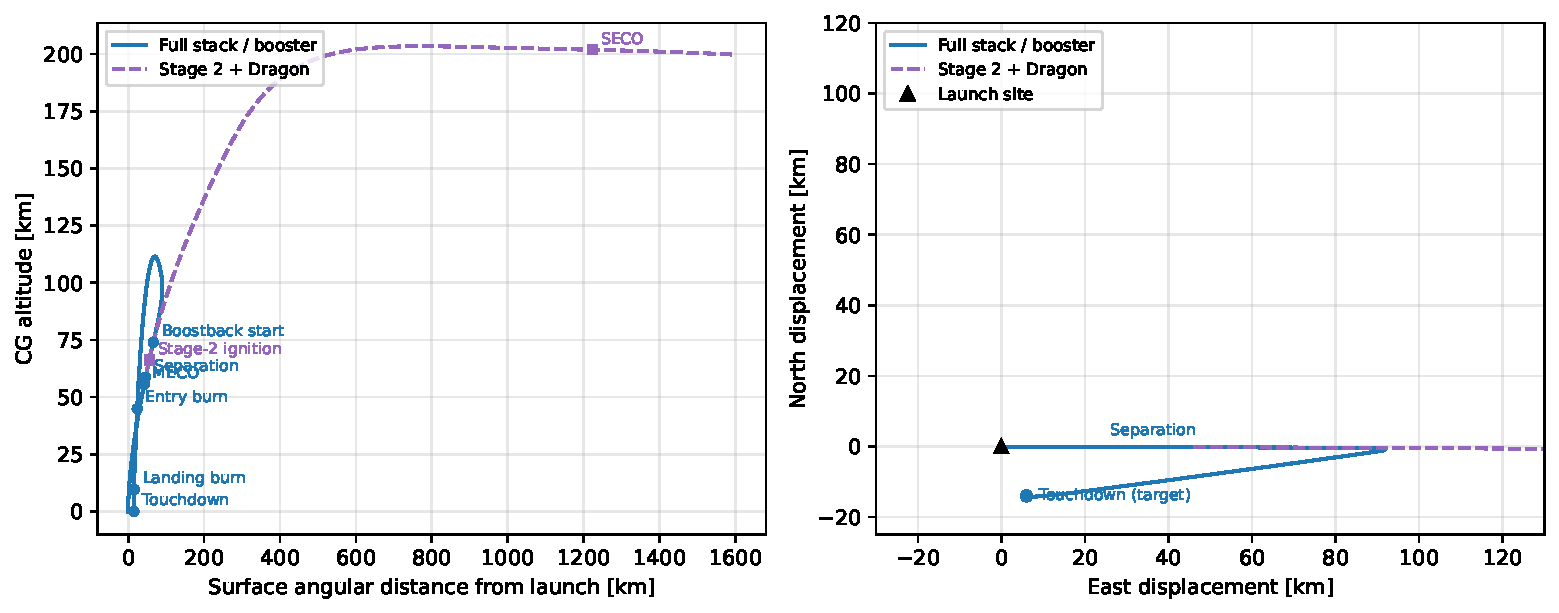
\includegraphics[width=\linewidth]{images/flight_paths.pdf}
\caption{Simulated flight paths of the nominal full-mission run (seed~1).
Left: CG altitude against surface angular distance from the launch site.
Right: ground displacement; the launch site is at the origin and the
assumed landing target lies $14.0\,\mathrm{km}$ south and
$6.0\,\mathrm{km}$ east of it. Markers denote mission events.}
\label{fig:flightpaths}
\end{figure}
